
%%%%%%%%%%

%\begin{figure}[h]

\centering
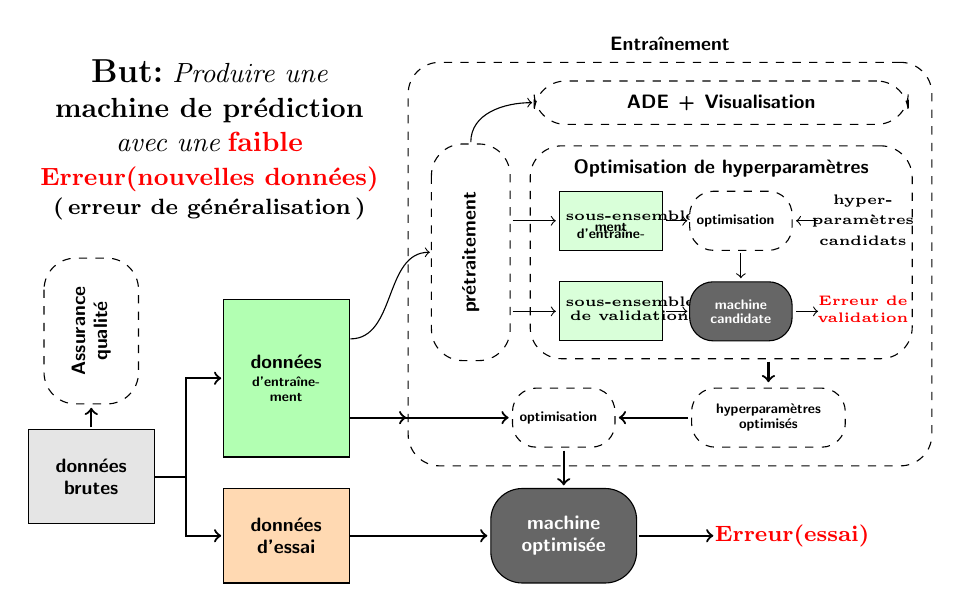
\begin{tikzpicture}
[node distance = 1cm, auto,font=\scriptsize,
% STYLES
every node/.style={node distance=3cm},
% The comment style is used to describe the characteristics of each force
comment/.style={rectangle, inner sep= 5pt, text width=4cm, node distance=0.25cm, font=\scriptsize\sffamily},
% The force style is used to draw the forces' name
force/.style={rectangle, draw, fill=black!10, inner sep=5pt, text width=1.25cm, text badly centered, minimum height=1.2cm, font=\bfseries\scriptsize\sffamily}] 

\pause
%\node at (1.5,6.6) {\large\bf Goal:\;\normalsize To produce};
%\node at (1.5,6.1) {\normalsize\bf a \it prediction machine};
%\node at (1.5,5.7) {\normalsize\bf with {\color{red}small}};
%\node at (1.5,5.225) {\normalsize\bf\color{red}Error(new data)};
\node at (1.5,6.9) {\large{\bf But:}\;\normalsize\it Produire une};
\node at (1.5,6.4) {\normalsize \bf machine de pr\'ediction};
\node at (1.5,6.0) {\normalsize \it avec une\;{\color{red}\bf faible}};
\node at (1.5,5.525) {\normalsize\bf\color{red}{\small Erreur(nouvelles donn\'ees)}};
\node at (1.5,5.15) {\footnotesize\bf(\,erreur de g\'en\'eralisation\,)};

%%%  ~~~~~~~~~~  %%%

\pause
\node [force] at (0,1.75) {donn\'ees brutes};

\pause
\draw [->,thick] (0,2.375) -- (0,2.625);
%\node [force, rotate=90, dashed, fill=white, rounded corners=0.4cm, text width=1.5cm] at (0,3.6) {Quality\\Assurance};
\node [force, rotate=90, dashed, fill=white, rounded corners=0.4cm, text width=1.5cm] at (0,3.6) {Assurance\\qualit\'e};

\pause
\draw [-,thick] (0.8,1.75) -- (1.2,1.75);
\draw [-,thick] (1.2,3) -- (1.2,1);
\draw [->,thick] (1.195,3) -- (1.65,3);
\draw [->,thick] (1.195,1) -- (1.65,1);

%\node [force, fill=green!30, minimum height=2cm, text width=1.25cm] at (2.475,3) {donn\'ees\\d'appren-\\tissage};
\node [force, fill=green!30, minimum height=2cm, text width=1.25cm] at (2.475,3) {donn\'ees\vskip 0.02cm \tiny d'entra\^ine-\vskip -0.1cm ment};
\node [force, fill=orange!30,text width=1.25cm] at (2.475,1) {donn\'ees\\d'essai};

%%%  ~~~~~~~~~~  %%%

\pause
\draw [->,thick] (3.29,2.5) -- (4.0,2.5);
\node [font=\bfseries\scriptsize\sffamily] at (7.35,7.25) {Entra\^inement};
\node [force, dashed, minimum height=5.125cm, text width=6.3cm, fill=white, rounded corners=0.4cm] at (7.35,4.45) {};

%%%  ~~~~~~~~~~  %%%

\pause
\draw [->,thick] (6,1.875) -- (6,1.64);
\node [force, text width=1.5cm, fill=black!60, rounded corners=0.4cm] at (6,1) {\color{white}machine\\optimis\'ee};

\pause
\draw [->,thick] (3.29,1) -- (5.03,1);
\draw [->,thick] (6.96,1) -- (7.9,1);
\node at (8.9,1) {\footnotesize\bf\color{red}Erreur(essai)};

%%%  ~~~~~~~~~~  %%%

\pause
%\draw [->,dashed] (3.29,3.5) to [out=0,in=180] (4.3,4.6);
\draw [->] (3.29,3.5) to [out=0,in=180] (4.3,4.6);
\node [force, dashed, rotate=90, minimum height=1.00cm, text width=2.4cm, fill=white, rounded corners=0.4cm] at (4.82,4.6) {
	pr\'etraitement %preprocessing
	};

%%%  ~~~~~~~~~~  %%%

\pause
%\draw [->,dashed] (4.82,6.00) to [out=90,in=180] (5.6,6.5);
\draw [->] (4.82,6.00) to [out=90,in=180] (5.6,6.5);
\node [force, dashed, minimum height=0.5cm, text width=4.4cm, fill=white, rounded corners=0.4cm] at (8.0,6.5) {
	ADE\;\,+\;\,Visualisation
	};

%%%  ~~~~~~~~~~  %%%

\pause
%\node [force, dashed, minimum height=2.125cm, text width=4.5cm, fill=white, rounded corners=0.4cm] at (8.0,4.75) {
\node [force, dashed, minimum height=2.125cm, text width=4.5cm, fill=white, rounded corners=0.4cm] at (8.0,4.6) {
	Optimisation de hyperparam\`etres\vskip 1.9cm{\color{white}1}
	};
%\draw [->,dashed] (5.25,5.00) to (5.9,5.00);
%\draw [->,dashed] (5.25,3.85) to (5.9,3.85);
\draw [->] (5.35,5.00) to (5.9,5.00);
\draw [->] (5.35,3.85) to (5.9,3.85);

%%%  ~~~~~~~~~~  %%%

\pause
\draw [->,thick] (8.6,3.21) -- (8.6,2.95);
\node [force, dashed, fill=white, minimum height=0.75cm, text width=1.6cm, rounded corners=0.3cm] at (8.6,2.5) {
	\tiny hyperparam\`etres\vskip -0.1cm optimis\'es
	};

\pause
\draw [->,thick] (3.97,2.5) -- (5.3,2.5);
\draw [->,thick] (7.58,2.5) -- (6.7,2.5);
\node [force, dashed, fill=white, minimum height=0.75cm, text width=0.95cm, rounded corners=0.3cm] at (6,2.5) {
	\!\!\!\tiny optimisation
	};
\draw [-,thick] (6,2.08) -- (6,1.7);

%%%  ~~~~~~~~~~  %%%

\pause
\node at (9.8,5.25) {\tiny\bf hyper-};
\node at (9.8,5.00) {\tiny\bf param\`etres};
\node at (9.8,4.75) {\tiny\bf candidats};

\pause
\node [force, fill=green!15, minimum height=0.75cm, text width=0.95cm] at (6.6,5.00) {
	\tiny \!\!\!$^{\textnormal{\bf sous-ensemble}}$
	\vskip -0.05cm d'entra\^ine-\vskip -0.375cm ment
	};
\node [force, fill=green!15, minimum height=0.75cm, text width=0.95cm] at (6.6,3.85) {
	\tiny \!\!\!$^{\textnormal{\bf sous-ensemble}}$
	\vskip -0.1cm$^{\textnormal{\bf\!de validation}}$
	};

\pause
%\draw [->,thick] (7.3,5.00) -- (7.57,5.00);
%\draw [->,thick] (9.23,5.00) -- (8.95,5.00);
\draw [->] (7.3,5.00) -- (7.57,5.00);
\draw [->] (9.23,5.00) -- (8.95,5.00);
\node [force, dashed, fill=white, minimum height=0.75cm, text width=0.95cm, rounded corners=0.3cm] at (8.25,5.00) {
	\!\!\!\tiny optimisation
	};

\pause
%\draw [->,thick] (8.25,4.59) -- (8.25,4.27);
\draw [->] (8.25,4.59) -- (8.25,4.27);
\node [force, fill=black!60, minimum height=0.75cm, text width=0.95cm, rounded corners=0.3cm] at (8.25,3.85) {
	\color{white}\tiny machine\vskip -0.1cm candidate
	};

\pause
%\draw [->,thick] (7.3,3.85) -- (7.57,3.85);
%\draw [->,thick] (8.95,3.85) -- (9.23,3.85);
\draw [->] (7.3,3.85) -- (7.57,3.85);
\draw [->] (8.95,3.85) -- (9.23,3.85);
\node at (9.8,3.98) {\color{red}\tiny\bf Erreur de};
\node at (9.8,3.77) {\color{red}\tiny\bf validation};
%\draw [<->,thick] (7.6,3) to [out=0,in=0] (7.6,4);
%\draw [<->,thick] (5.9,3) to [out=180,in=180] (5.9,4);

%%%%%%%%

\end{tikzpicture}

%%%%%%%%%%
